\section{Concepts}
In this section, important theoretical concepts will be explained using a simple traffic light example. They must be clearly understood in order to ensure that our project reaches the required level of success. We will discuss about timed automata, temporal logic and their properties, and game theory to reach a winning condition.

\subsection{Timed Automata} \label{sec:automate}
A timed automaton is essentially a finite automaton (that is a graph
containing a finite number of nodes and labeled edges) extended with real-valued variables. Those automata run on an infinite words as input and they accept timed languages. The variables that exist in the model can represent logical clocks of the system that will be increased synchronously with the same rate.
It is possible to add constraints called \textbf{guards} on the edges to create restriction on our automaton. A transition could thus occur when the value of the clock satisfy the guard's condition on the edge.

\begin{figure}[H]\label{fig:timed}
  \centering
    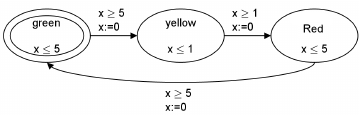
\includegraphics[width=0.7\textwidth]{picture/trafficlight.png}
    \caption{A timed automaton example}
\end{figure}

The example of Figure \ref{fig:timed} represent a basic light example where the light goes from the green state to the yellow state if the clock is higher or equal to 5. It then resets the clock to 0 and stays in the yellow state for a time lower or equal to one. When the clock has an higher value, it switches to the red state and so on.

\subsection{Temporal Logic and Properties}
The aim of temporal logic is to become a formalism of specification and verification of some properties in reactive systems. In our case, two different kind of logic will be of interest: \textbf{Linear Temporal Logic (LTL)} and \textbf{Computation Tree Logic (CTL)}. Those two kind of logic are only concerned with infinite paths. They, for example, allow us to make statements, such as "Tomorrow, something will eventually be true". Thanks to this, we can define specific properties our system has to comply to. \\
There are of course differences between the two. In the first kind of logic, the LTL one, we will look at the traces of executions, meaning that we will look at the states we reach in a linear manner.
If we look back at Figure \ref{fig:timed}, the traces would be:\\ ${Green \rightarrow Yellow \rightarrow Red \rightarrow Green \rightarrow Yellow \rightarrow Red \rightarrow Green \rightarrow ...}$. \\
In the other kind of logic, the CTL one, we will use a branching time semantic instead of a linear semantic. Here, the different execution (or computation) trees will be considered for all branching possibilities. \\
An example of propriety we can verify thanks to CTL and that is not possible to verify in LTL is "do all executions always have the possibility to eventually reach a certain state". Indeed, intuitively it would require branching to verify it. \\
The following temporal properties can be expressed using either CTL or LTL:
\begin{itemize}
    \item Safety: The system never reaches an unwanted state (CTL and LTL)
    \item Liveness: Ensure that our system will reach a certain state infinitely often, meaning that no deadlocks can occur (CTL and LTL)
    \item Fairness: Everyone is at some point satisfied (LTL and CTL)
    \item Persistence: Ensure that a property eventually holds forever (only LTL)
\end{itemize}

\subsection{Game Theory and Timed Games} \label{sec:game}
Game theory can be defined as the formal study of decision-making where several players must make choices that potentially affect the interests of the other players\footnote{\url{http://www.cdam.lse.ac.uk/Reports/Files/cdam-2001-09.pdf}}. As when playing a game, we would want to find a winning situation. In our case, there will be two different type of players. The first one will be the controller, something that we can control and define, while the second one, his opponent thus, will be called the environment. \\

The traffic lights will be the first player (the controller since we can control it) while the buses and the pedestrians will be the second player. Since the buses and pedestrians are playing when an external event occurs (a button that is pushed), they will be the environment. The main goal of the controller will be to find a winning strategy in this game, being a sequence of moves that will inevitably lead to the wanted outcome. In our case, we would want the lights to respect the properties that we have defined, even when pedestrians want to cross the street or buses want to go through the crossroad. If at some point all the traffic lights for the cars are green, it would mean that the system is broken and that the controller has lost the game. This is a situation we would not want to happen. \\

\textbf{Times Games} is an important part of the game and the rules, it brings a real-time dimension. An example of a timed game can be a chess game, where all the two players have to make a move within a given time. In our case, the controller that is the traffic light has to keep the buses, the cars and the pedestrians safe while taking into account the time constraints on the traffic lights.
